\documentclass[10pt,letterpaper,notitlepage]{article}
\usepackage[utf8]{inputenc}
\usepackage[T1]{fontenc}
\usepackage{amsmath,amsfonts,amssymb}
\usepackage{caption,graphicx}
\usepackage{hyperref,cleveref}
\usepackage{derivative}
\usepackage{changepage}
\usepackage[backend=biber]{biblatex}
% \addbibresource{hw4.bib}
\DeclareCaptionFormat{plain}{%
  \fbox{\parbox{\dimexpr\linewidth-2\fboxsep-2\fboxrule}{ #1#2#3}}}

\author{Mike Sutherland}
\title{MAE 195 Final Project S22}
\begin{document}
    \maketitle
    \section{Part A}
    \label{sec:parta}
    We have a steady state non-dimensional heat equation given by
    \begin{equation}
        \frac{d^2 \theta}{d\xi^2} - \beta \theta = -\beta \theta_f
        \label{eq:ss}
    \end{equation}
    Where $\theta_f$ does not depend on $\xi$. The exact solution is a function of the parameters $\beta$ and $\theta_f$. The solution of this equation takes the form:
    \begin{equation}
        \theta(\xi) = c_1 e^{\sqrt{\beta} \xi} + c_1 e^{-\sqrt{\beta} \xi} - \frac{\theta_f}{\beta}
    \end{equation}
    The exact analytic solution can be found for a particular pair of boundary conditions $\theta(\xi_1)$ and $\theta(\xi_2)$ by solving the system given by:
    \begin{equation}
        \begin{bmatrix}
            e^{\sqrt{\beta} \xi_1} & e^{-\sqrt{\beta} \xi_1} \\
            e^{\sqrt{\beta} \xi_2} & e^{-\sqrt{\beta} \xi_2} 
        \end{bmatrix}
        \begin{bmatrix}
            c_1 \\
            c_2
        \end{bmatrix}
        =
        \begin{bmatrix}
            \theta(\xi_1) \\
            \theta(\xi_2)
        \end{bmatrix}
    \end{equation}
    For the coefficients $c_1$, $c_2$.

    We can obtain a numerical approximation of \cref{eq:ss} at a grid point $i$ by replacing the derivative term with a finite difference approximation over a grid with spacing $h$:
    \begin{equation}
        \frac{d^2 \theta_i}{d\xi^2} = \frac{ \theta_{i-1} - 2 \theta_i + \theta_{i+1} }{h^2} + \mathcal{O}(h^2)
        \label{eq:finitediff2}
    \end{equation} 
    Substituting \cref{eq:finitediff2} into \cref{eq:ss} yields:
    \begin{align}
        \frac{\theta_{i-1}}{h^2} + \frac{-2 \theta_i}{h^2} + 
        \frac{\theta_{i-1}}{h^2} + \mathcal{O}(h^2) - \beta{\theta_i} 
        &= -\beta \theta_{i,f}\\
        \left(\frac{-1}{h^2}\right) \theta_{i-1} + 
        \left(\frac{2}{h^2} + \beta \right) \theta_{i} + 
        \left(\frac{-1}{h^2}\right) \theta_{i+1} +
        \mathcal{O}(h^2)
        &= \beta \theta_{i,f}
        \label{eq:Amatrixeqn}
    \end{align}
    Using this equation, we can obtain a numerical approximation for each interior grid point $i$. For a grid with step size $h=\frac{1}{6}$, we have $n=6$ grid points, $n=4$ of which are internal grid points. We will use a zero-indexed notation for the grid points. In this case, $\theta$ is known at the endpoints, $i=0$ and $i=5$. We can construct the matrix system $[A] \{\theta\} = \{b\}$ as follows.
    \begin{equation}
        \begin{bmatrix}
            1 & 0 & 0 & 0 & 0 & 0 \\
            -\frac{1}{h^2} & \frac{2}{h^2} + \beta & -\frac{1}{h^2} & 0 & 0 & 0 \\
            0 & -\frac{1}{h^2} & \frac{2}{h^2} + \beta & -\frac{1}{h^2} & 0 & 0 \\
            0 & 0 & -\frac{1}{h^2}& \frac{2}{h^2} + \beta & -\frac{1}{h^2} & 0 \\
            0 & 0 & 0 & -\frac{1}{h^2} & \frac{2}{h^2} + \beta & -\frac{1}{h^2} \\
            0 & 0 & 0 & 0 & 0 & 1 
        \end{bmatrix}
        \begin{bmatrix}
            \theta_0 \\
            \theta_1 \\
            \theta_2 \\
            \theta_3 \\
            \theta_4 \\
            \theta_5
        \end{bmatrix}
        =
        \begin{bmatrix}
            \theta(\xi_0) \\
            \theta_f \\
            \theta_f \\
            \theta_f \\
            \theta_f \\
            \theta(\xi_5)  
        \end{bmatrix}
        \label{eq:ss_Axb}
    \end{equation}
    \begin{figure}
        \centering
        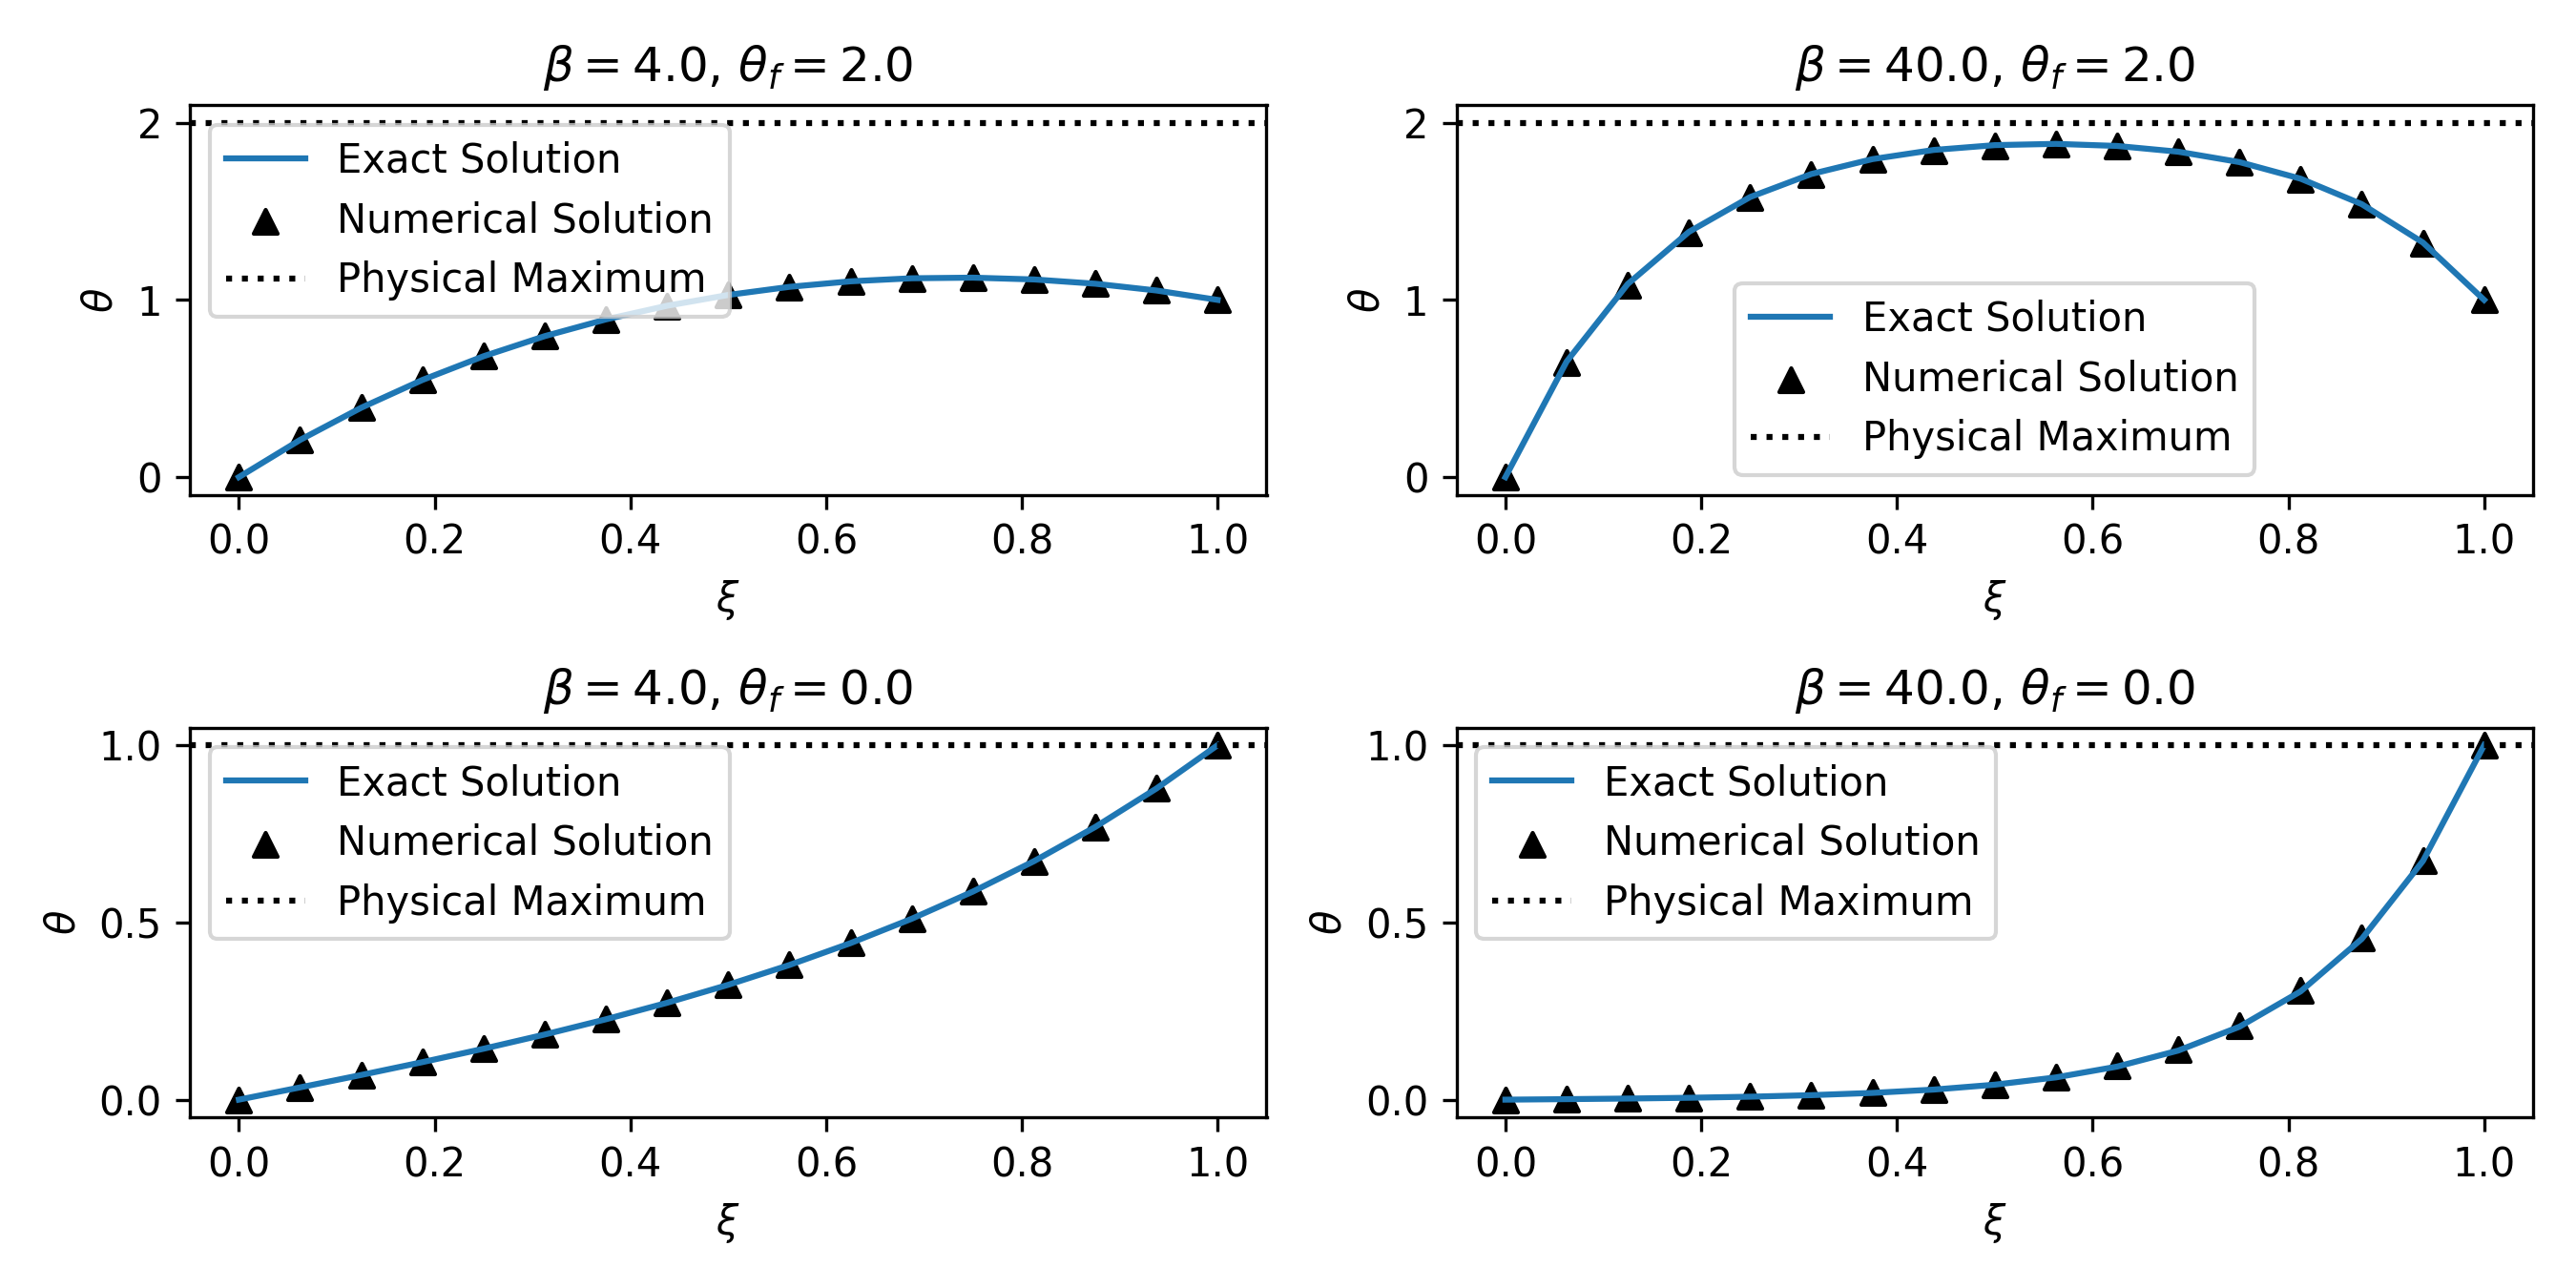
\includegraphics[width=\textwidth]{figures/Temperature Distributions for Different Parameters.png}
        \caption{Temperature distributions for different parameters. The maximum physicaly possible temperature in the fin is less than or equal to the temperature of the free fluid, or the temperature of the fin at its boundary condition, whichever is less. The maximum physically possible temperature can be seen by the dashed line. The dimensionless parameter $\beta \propto \frac{1}{k}$ represents the conductivity of the material. The dimensionless $\theta_f$ is the uniform temperature of the free stream. We see that higher values of $\beta$ correpond to the behavior of a less conductive fin, as we expect.}
        \label{fig:TemperatureDistributions}
    \end{figure}
    This tridiagonal system can be solved quickly using the Thomas algorithm (TDMA) to obtain the full vector of temperatures. The solution for this system for several parameters is shown in \cref{fig:TemperatureDistributions}
    \begin{figure}
        \centering
        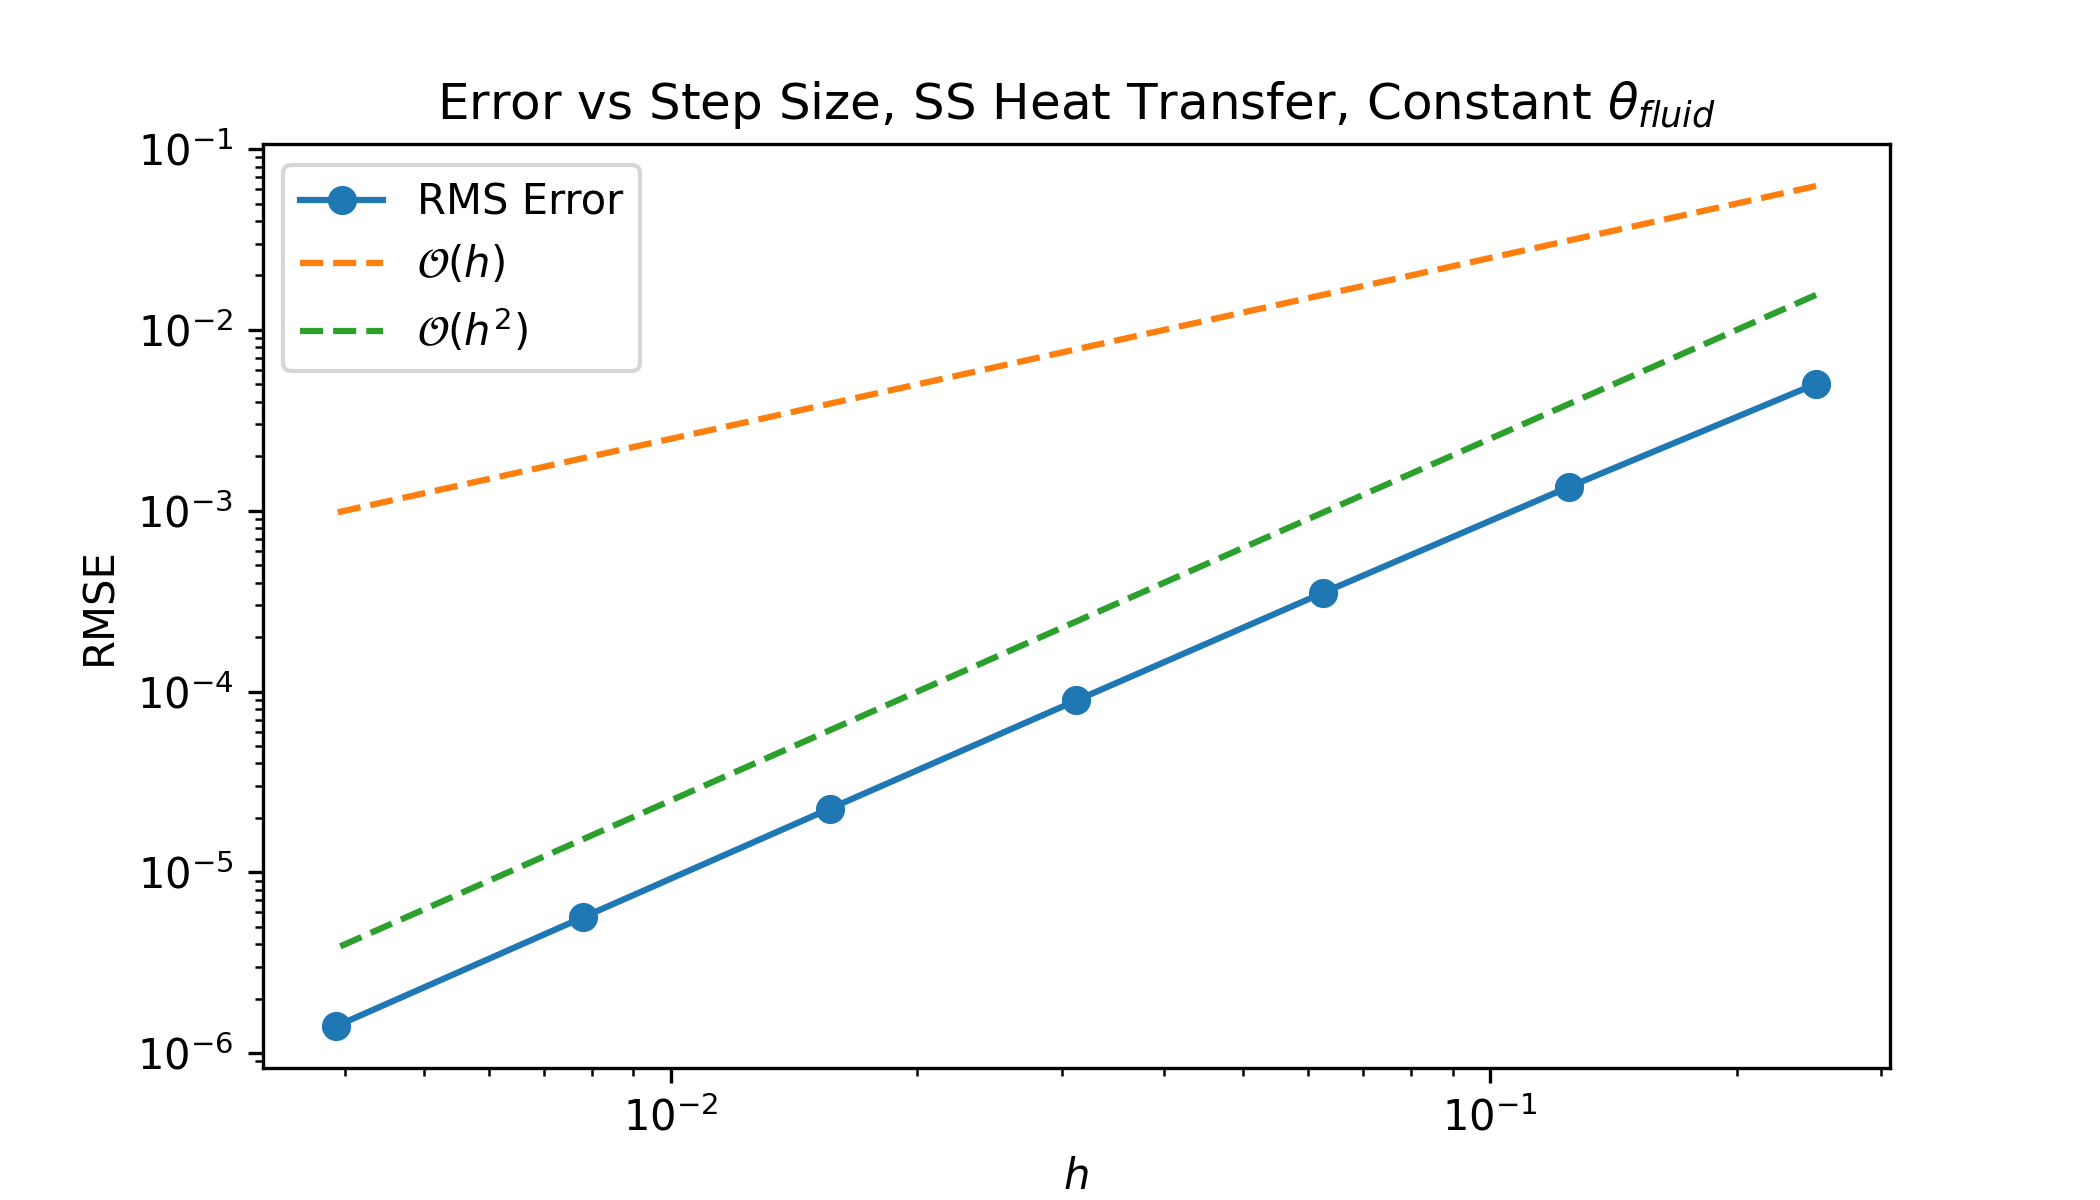
\includegraphics[width=0.8\textwidth]{figures/RMS Error vs h.png}
        \caption{The root mean squared error (RMSE) for a variety of grid spacings $h$. We can see that the approximation used in \cref{eq:Amatrixeqn} has truncation error on the order of $\mathcal{O}(h^2)$, as we expect.}
        \label{fig:RMSError}
    \end{figure}
    We compare the finite difference approximation to the exact solution for various grid sizes in \cref{fig:RMSError} and verify that the error is $\mathcal{O}(h^2)$. 
    \subsection{Part 5}
    Consider a control volume that encloses the fin. We have two areas through which heat can pass: the fin surface, exposed to the fluid, and the fin ends, which are attached to some solid substrate. The heat flux through the fin surface occurs via convection, and the heat flux through the fin ends occurs via conduction. If we assume that no energy is generated inside of the fin, the total heat flux is given by:
    \begin{equation*}
        Q = Q_{\text{cond}} + Q_{\text{conv}} = 0
    \end{equation*}
    Then, we can say that 
    \begin{equation*}
        Q_{\text{cond}} = -Q_{\text{conv}}
    \end{equation*}
    That is, depending on the fluid temperature, heat travels from the substrate, through the fin, and into the fluid, consistent with a cooling application. To evaluate the transfer by convection, we have that:
    \begin{equation}
        Q_{\text{conv}} = \int_{0}^{L} h (T-T_f) dx
    \end{equation}
    Where $h$ is the coefficient of convection (not grid spacing!). We can non-dimensionalize to obtain the conduction term:
    \begin{equation}
        \beta \int_{0}^{1}(\theta - \theta_f) d\xi
        \label{eq:convterm}
    \end{equation}
    The convection term is modeled by Newton's law of cooling:
    \begin{equation*}
        k A (\left. \frac{dT}{dx} \right|_{0} - \left. \frac{dT}{dx} \right|_{L}) = 0
    \end{equation*}
    which can be non-dimensionalized:
    \begin{equation}
        \left. \frac{d\theta}{d\xi} \right|_{0} - \left. \frac{d\theta}{d\xi} \right|_{1}
        \label{eq:condterm}
    \end{equation}
    If the energy balance is to hold, we have then that convection out of the control volume (\cref{eq:convterm}) equals conduction into the control volume (\cref{eq:condterm}):
    \begin{equation}
        0 = \left. \frac{d\theta}{d\xi} \right|_{0} - \left. \frac{d\theta}{d\xi} \right|_{1} + \beta \int_{0}^{1}(\theta - \theta_f) d\xi
    \end{equation}
    The convection term can be obtained via integration of the temperature profile. We can use the analytic solution to (\cref{eq:ss}) to obtain the temperature profile. Then, we can numerically integrate.

    \begin{figure}
        \centering
        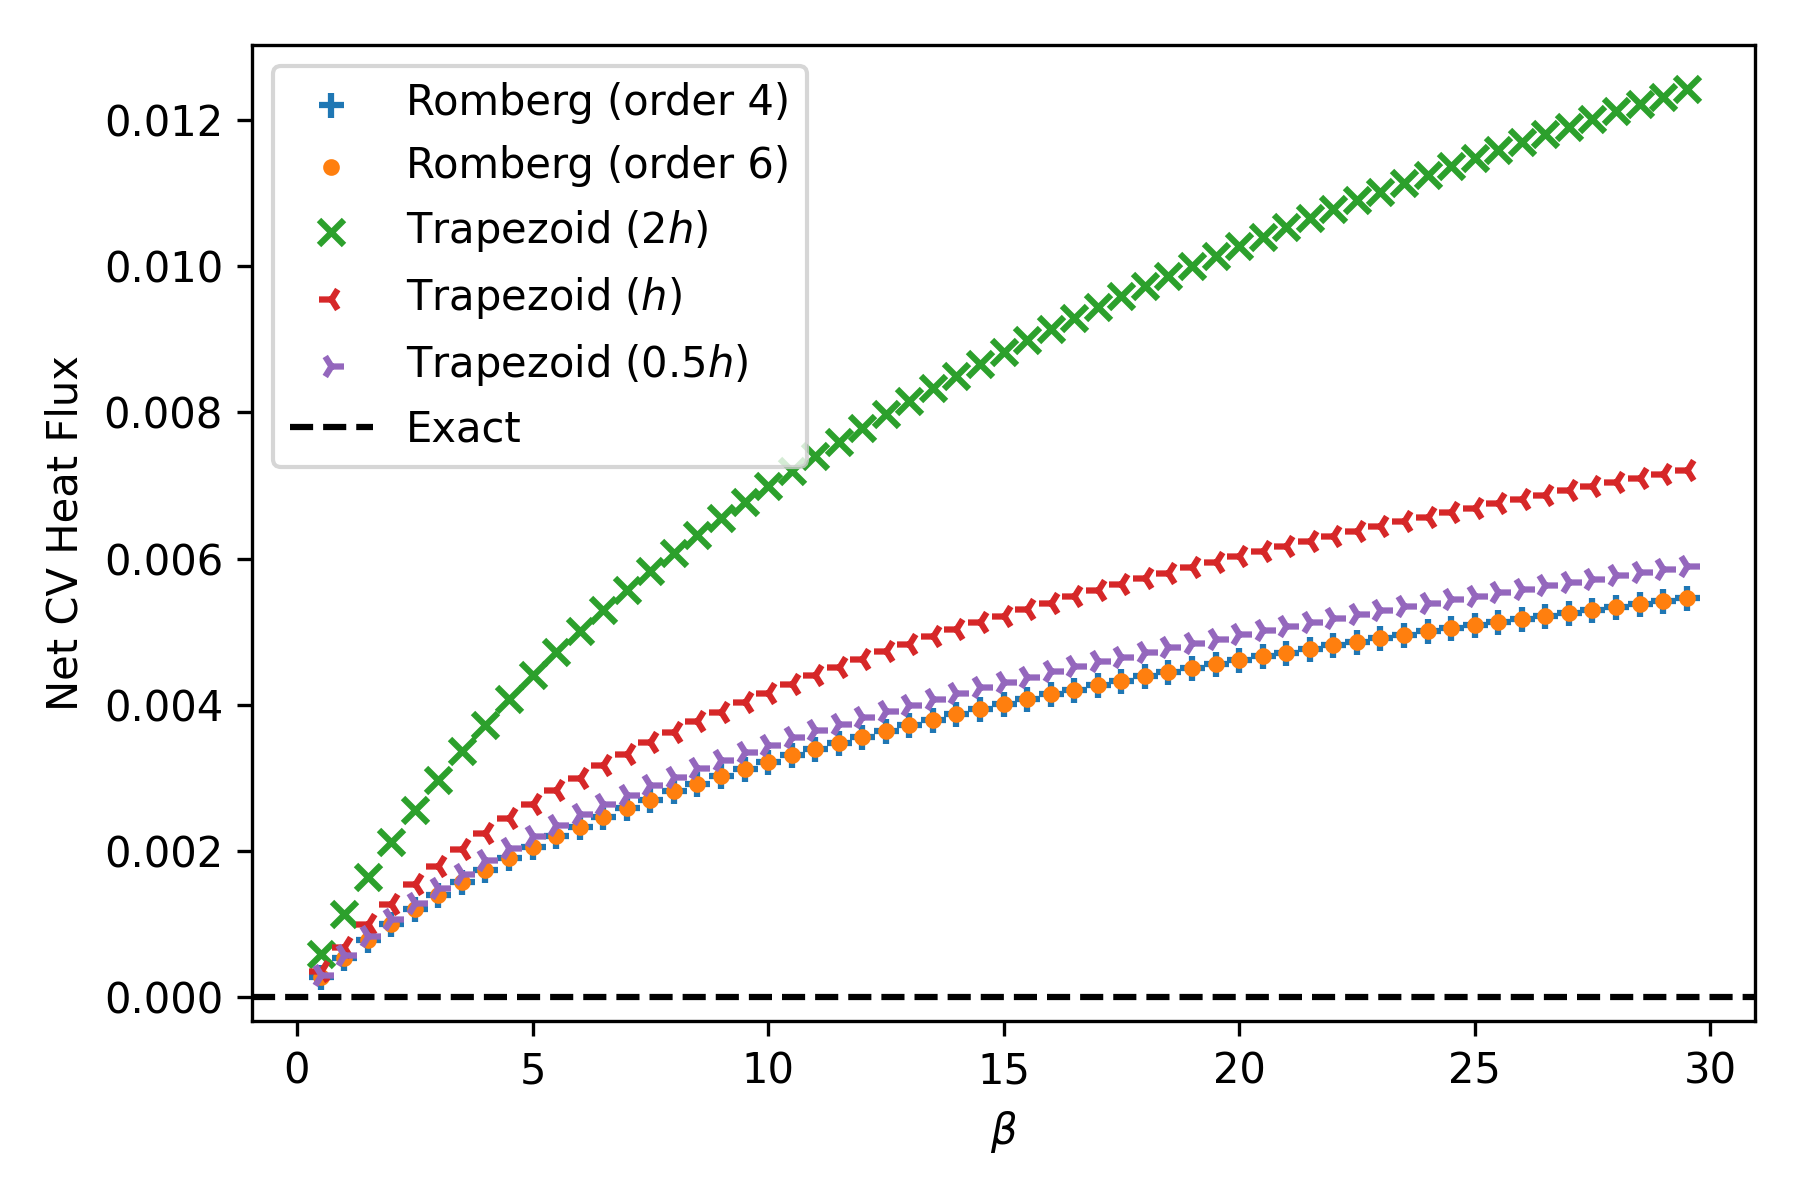
\includegraphics[width=0.8\textwidth]{figures/Heat Flux, Step Size, beta.png}
        \caption{The error in control volume heat flux as a function of $\beta$ for various methods of integration. The lower truncation error of the romberg methods is apparent in the plot; it is lower than that of composite trapezoid integration. However, there is a diminishing return; even though the order-6 Romberg integration is more accurate than the order-4 Romberg integration, the $\mathcal{O}(h^2)$ error of the finite difference method used in the conduction term begins to dominate. In order to achieve a lower error for the heat flux in the control volume, we would need to use a higher-order method for the differentiation term.}
        \label{fig:integration5}
    \end{figure}

    Integration to solve convection was carried out using the trapezoid rule for $h=\frac{1}{8}$, $h=\frac{1}{16}$, and $h=\frac{1}{32}$. Additionally, a $\mathcal{O}(h^4)$ and $\mathcal{O}(h^6)$ romberg method was used.

    Meanwhile, differentiation to solve conduction was kept steady at a 2nd-order method for each boundary point.

    Then, a series of problems with varying $\beta$ values were solved. Because the convection term depends on $\beta$, the accuracy of an integration methods will depend not only on $h$, but also on $\beta$. The results are shown in \cref{fig:integration5}.

    \section{Part B}
    Now, we consider a problem where the free stream temperature is a function of its station along the fin: $\theta_f = f(\xi)$. We consider a gaussian "plume" of high temperature in the free stream, given by the function:
    \begin{equation}
        f(\xi) = A \exp{\left( \frac{-(\xi - \xi_0)^2}{2 \sigma^2} \right)}
    \end{equation}
    The plume has magnitude $A$, is centered at $\xi_0$, and has a width corresponding to $\frac{1}{\sigma ^2}$.
    \begin{figure}
        \centering
        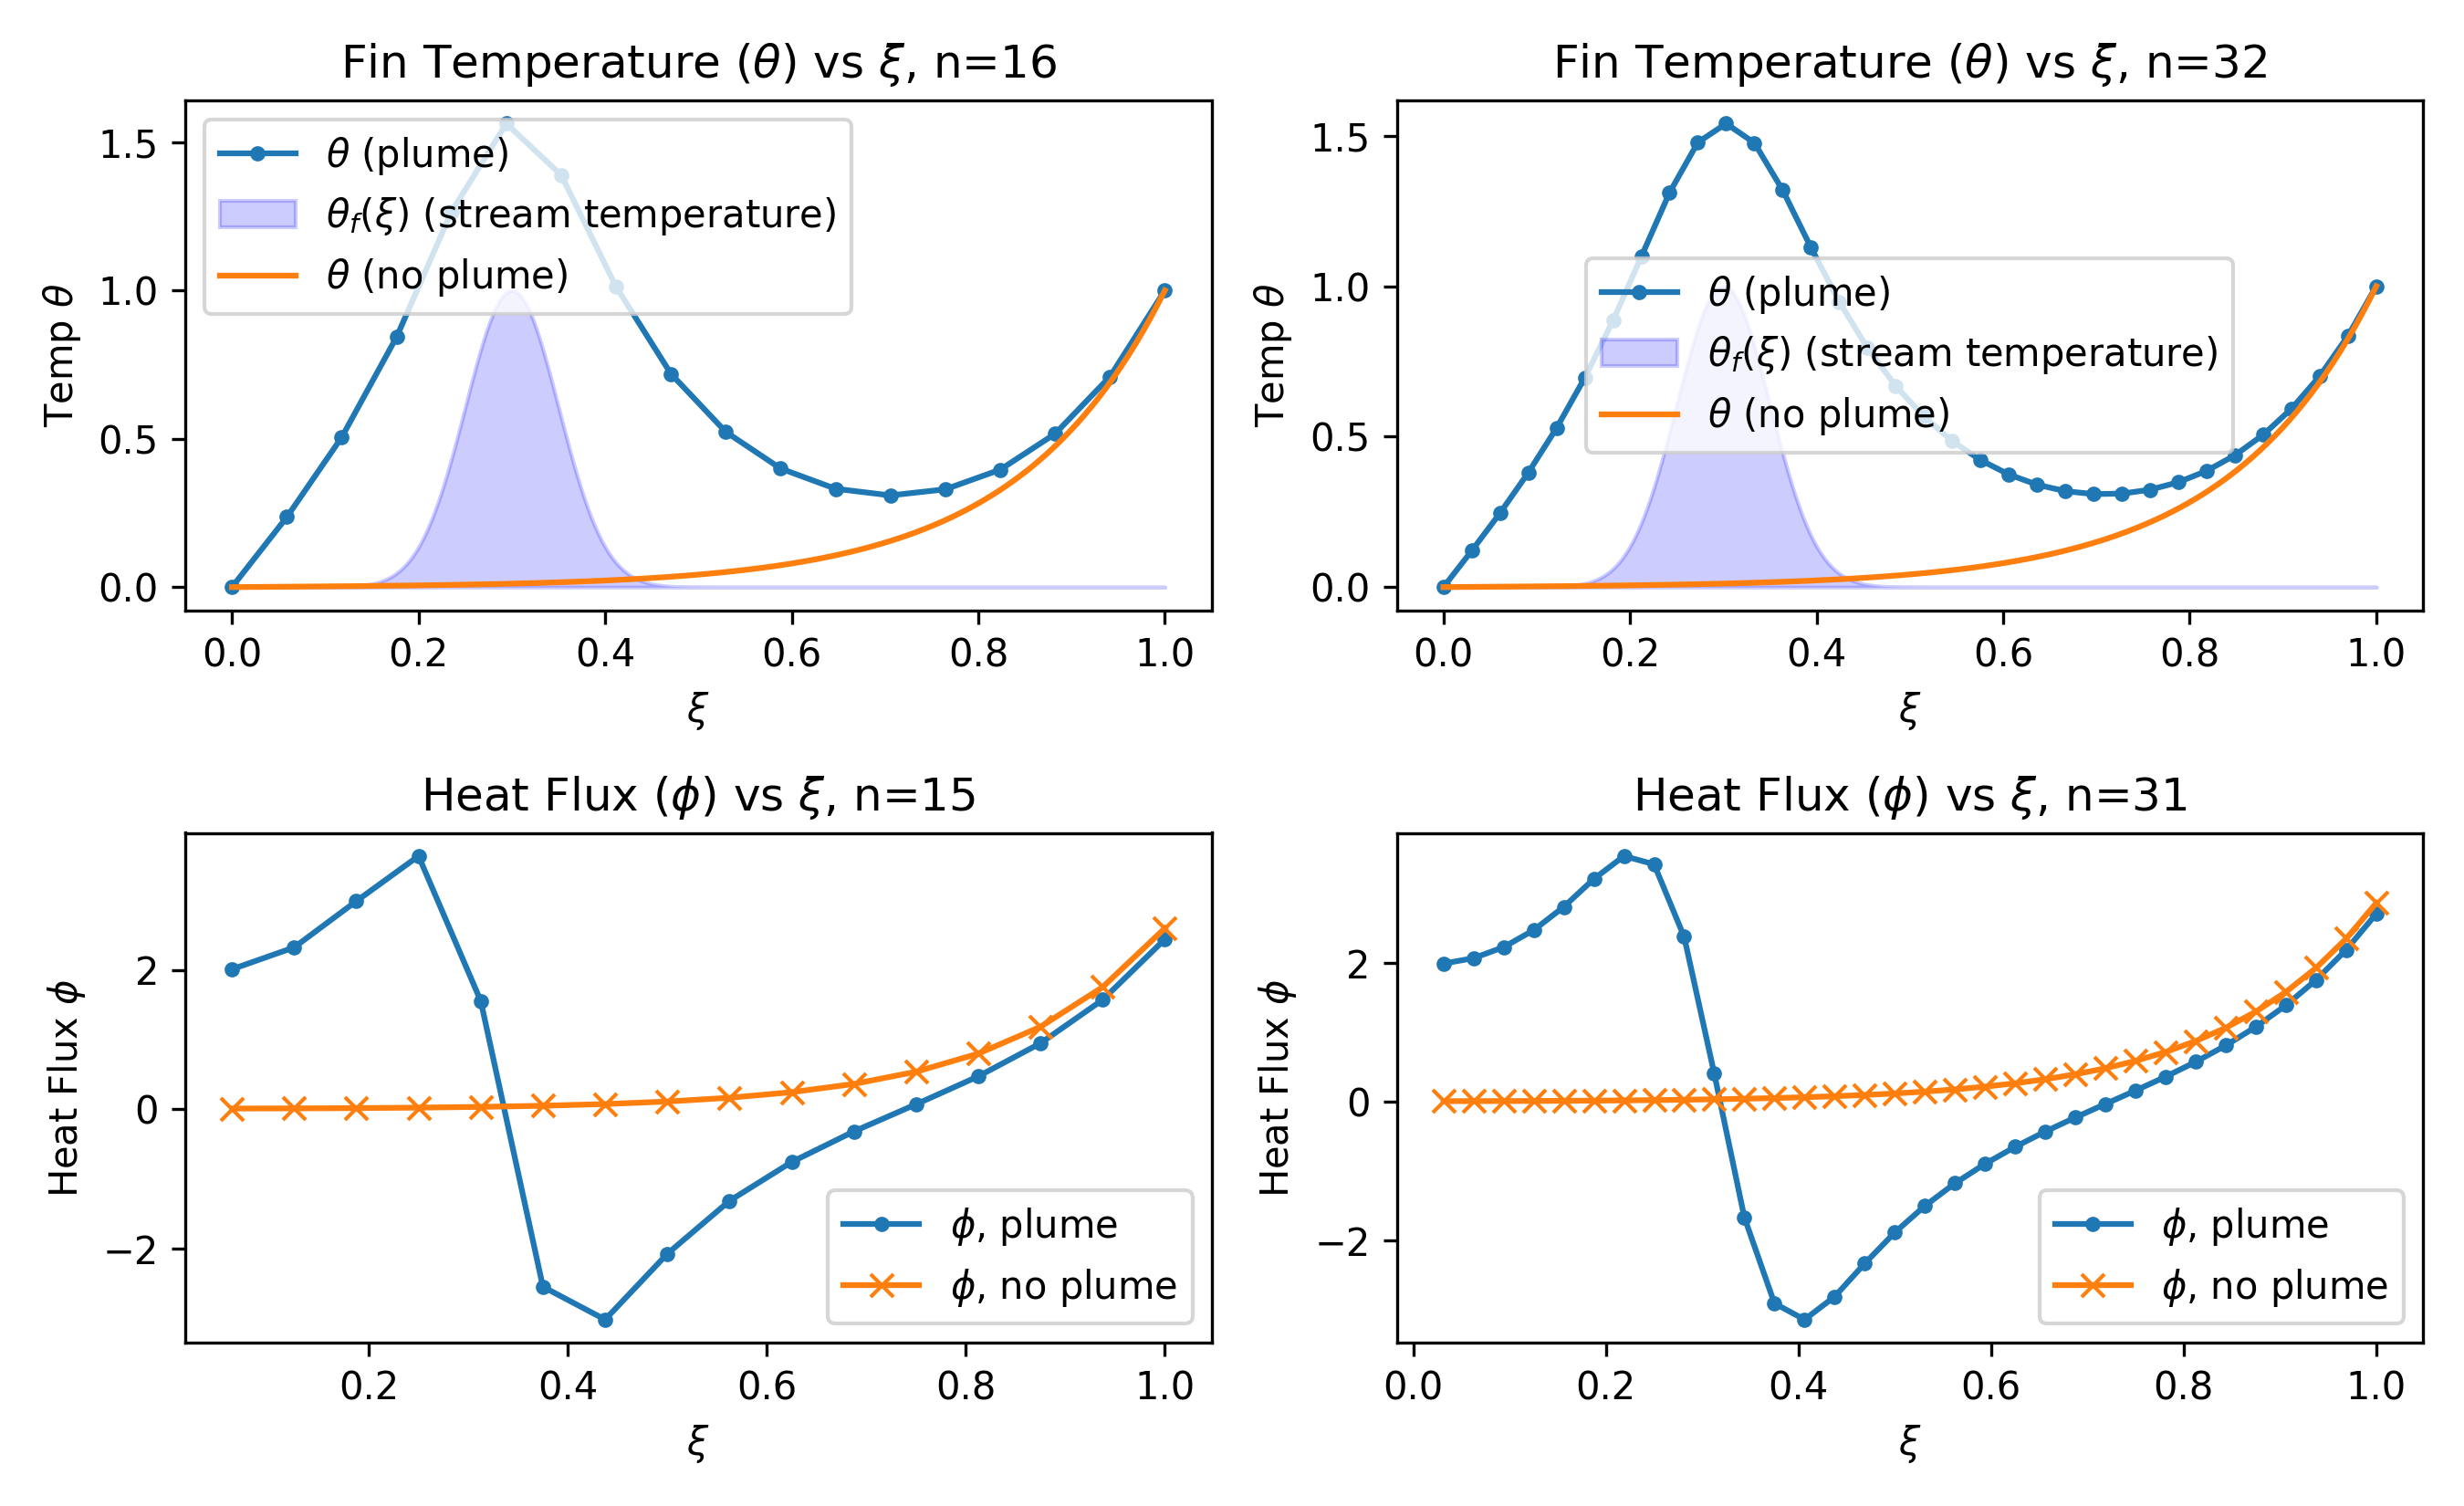
\includegraphics[width=\textwidth]{figures/plume.png}
        \caption{Numerical solution of the $\theta_f = f(\xi)$ fluid profile (blue) and the $\theta_f = 0$ fluid profile (orange). The temperature of the fluid is shown in red. On the top row, we have fluid temperature vs $\xi$. We can see that where the fluid is the highest temperature, the temperature of the fin commensurately rises. Bottom row shows heat flux. The heat energy passing into the fin from the plume flows through the fin towards the cold areas of the fluid, and towards the cold left boundary.}
        \label{fig:plume}
    \end{figure}
    Although finding the analytic solution of the $\theta_f=f(\xi)$ problem may be difficult or impossible, the numerical solution is trivial: the procedure is the same regardless of the fluid temperature profile.
    \section{Part C}
    Now we change the conditions so that the fluid temperature is also a function of time.
    \begin{equation}
        \theta_f(\xi, \tau) = A \sin{\omega \tau} \exp{\left(\frac{-(\xi-\xi_0)^2}{2 \sigma ^2}\right)}
        \label{eq:thetaf_dynamic}
    \end{equation}
    This represents a fluid with a plume centered at $\xi_0$, the temperature of which oscillates between $A$ and $-A$ in a sinusoidal fashion with a period $\omega$.
    We can rewrite our governing equation:
    \begin{equation}
        \pdv{\theta}{\tau} = \pdv[2]{\theta}{\tau} + \beta (\theta_f - \theta)
        \label{eq:governing_time}
    \end{equation}
    We can give the RHS of this equation a similar treatment as in \cref{sec:parta}:
    \begin{align}
        \pdv{\theta}{\tau} &= \frac{\theta_{i-1}}{h^2} + \frac{-2 \theta_i}{h^2} + \frac{\theta_{i-1}}{h^2}+ \beta \left(\theta_{f,i} - \theta_i \right) + \mathcal{O}(h^2) \\
        \pdv{\theta}{\tau} &= 
        \left(\frac{1}{h^2}\right) \theta_{i-1} + 
        \left(\frac{-2}{h^2} - \beta \right) \theta_i +
        \left(\frac{1}{h^2}\right) \theta_{i+1} + 
        \left(\beta\right) \theta_{f,i,j} + 
        \mathcal{O}(h^2)
        \label{eq:explicit_time}
    \end{align}
    This produces a matrix equation similar to \cref{eq:Amatrixeqn}:
    \begin{equation}
        \pdv{\theta}{\tau} = -[A] \theta + b 
    \end{equation}
    This equation is nearly identical to that of the equation in \cref{sec:parta}.
    \begin{adjustwidth}{-1cm}{-1cm}
        \begin{equation}
            \pdv{\theta}{\tau}
            =
            \begin{bmatrix}
                1 & 0 & 0 & 0 & 0 & 0 \\
                \frac{1}{h^2} & -\frac{2}{h^2} - \beta & \frac{1}{h^2} & 0 & 0 & 0 \\
                0& \frac{1}{h^2} & -\frac{2}{h^2} - \beta & \frac{1}{h^2} & 0 & 0 \\
                0&0&\frac{1}{h^2} & -\frac{2}{h^2} - \beta & \frac{1}{h^2} & 0\\
                0&0&0&\frac{1}{h^2} & -\frac{2}{h^2} - \beta & \frac{1}{h^2} \\
                0 & 0 & 0 & 0 & 0 & 1 
            \end{bmatrix}
            \begin{bmatrix}
                \theta_{(0, j)} \\
                \theta_{(1, j)} \\
                \theta_{(2, j)} \\
                \theta_{(3, j)} \\
                \theta_{(4, j)} \\
                \theta_{(5, j)}
            \end{bmatrix}
            +
            \beta
            \begin{bmatrix}
                \theta_{(\xi=0,j)} \\
                \theta_{(f,1,j)} \\
                \theta_{(f,2,j)} \\
                \theta_{(f,3,j)} \\
                \theta_{(f,4,j)} \\
                \theta_{(\xi=1,j)}
            \end{bmatrix}
            \label{eq:td_Axb}
        \end{equation}
    \end{adjustwidth}
    With this formulation, we have the form $\pdv{\theta}{\tau} = f(\theta, \tau)$, which we can use any explicit method to solve.
    


    % \subsection{Explicit Method}
    % With this time-dependent equation, we have two dimensions: a time dimension $\tau$, and a spatial dimension, $\xi$. Therefore, we can re-write our equation with two dimensions, $i$ and $j$. We will label the grid spacing in the $j$-dimension as $t$. The $i,j$-th entry of our equation can thus be re-written in terms of its discrete temporal and spatial neighbors:
    % \begin{adjustwidth}{-1cm}{-1cm}
    % \begin{equation}
    %     \frac{-\theta_{i,j}+ \theta_{i,j+1} }{t} +\mathcal{O}(t) = \frac{\theta_{i-1,j}}{h^2} + \frac{-2 \theta_{i,j}}{h^2} + \frac{\theta_{i+1,j}}{h^2}+ \beta \left(\theta_{fluid \hspace{0.1cm} i,j} - \theta_{i,j} \right) + \mathcal{O}(h^2)
    %     \label{eq:fd_time}
    % \end{equation}
    % \end{adjustwidth}
    % The $\theta_{fluid \hspace{0.1cm} i,j}$ term, rather than being a steady-state function only of $\xi$, is now a function both of time and space, governed by \cref{eq:thetaf_dynamic}. Because we use a first-order finite-difference approximation in $\tau$, we have a corresponding first-order error in time.
    % We can re-arrange and simplify \cref{eq:fd_time}:
    % \begin{adjustwidth}{-2cm}{-2cm}
    % \begin{align}
    %     \frac{\theta_{i,j+1}}{t} &= \frac{\theta_{i,j}}{t} + \frac{\theta_{i-1,j}}{h^2} + \frac{-2 \theta_{i,j}}{h^2} + \frac{\theta_{i+1,j}}{h^2} - \beta \theta_{i,j} + \beta \theta_{fluid \hspace{0.1cm} i,j}  + \mathcal{O}(t) + \mathcal{O}(h^2) \\
    %     \theta_{i,j+1} &= \theta_{i,j} + t \frac{\theta_{i-1,j}}{h^2} + t \frac{-2 \theta_{i,j}}{h^2} + t \frac{\theta_{i+1,j}}{h^2} - t \beta \theta_{i,j} + t \beta \theta_{fluid \hspace{0.1cm} i,j}  + t \mathcal{O}(t) + t \mathcal{O}(h^2) \\
    %     \theta_{i, j+1} &= \left(\frac{t}{h^2}\right) \theta_{i-1,j} + \left( 1 - \frac{2 t}{h^2} - \beta t \right) \theta_{i,j} + \left(\frac{t}{h^2}\right) \theta_{i+1,j} + t \beta \theta_{fluid \hspace{0.1cm} i,j} + t \mathcal{O}(t) + t \mathcal{O}(h^2) 
    %     \label{eq:fd_time}
    % \end{align}
    % \end{adjustwidth}
    % This equation represents the relationship between a single grid point and all of its spatial and temporal neighbors. Notice that the state of a single grid point in the future ($j+1$) is dependent on both its state in the past ($i, j$), the effect of the fluid ($\theta_{(f, i, j)}$), and the prior state of its neighbors ($i-1, j$) and ($i+1, j$). Let us again write a matrix equation for $n=6$ system.
    % In this case, we have three different boundary conditions: in order to increment time, we need the first state, $j=0$, to be a fully fixed (steady state) condition. The second boundary condition is the left and right fin ends: $i=0$ and $i=n-1$, corresponding to $\xi=0$ and $\xi=1$. The final boundary condition is the space and time-dependent equation of the fluid, corresponding to $\left(i=1,i=2, ... i=n-2 \right)$.
    % Similar to \cref{eq:ss_Axb}, we can write \cref{eq:fd_time} in matrix form. For a single timestep, we have that 
    
    % This is a matrix equation of the form 
    % \begin{equation}
    %     \theta_{j+1} = [A] \theta_{j} + b_{j}
    % \end{equation}

    % Thus, the state of the system can be solved explicitly. We fix the entire $\theta$ vector at  $j=0$ by solving the steady state equation (whose form can be seen in \cref{eq:ss_Axb}). Then, to find some future state in time, we can get the time-dependent bounary condition $b_j$ and multiply the current state by A.

    % This has some remarkable stability downsides, which we will work around in \cref{sec:implicit}


    % \subsection{Implicit: Crank Nicholson}
    % \label{sec:implicit}




    



    % \printbibliography
    
\end{document}